\documentclass[a4paper, 10 pt, conference]{ieeeconf}
\overrideIEEEmargins

% The following packages can be found on http:\\www.ctan.org
%\usepackage{graphics} % for pdf, bitmapped graphics files
%\usepackage{epsfig} % for postscript graphics files
%\usepackage{mathptmx} % assumes new font selection scheme installed
%\usepackage{times} % assumes new font selection scheme installed
%\usepackage{amsmath} % assumes amsmath package installed
%\usepackage{amssymb}  % assumes amsmath package installed
\usepackage{graphicx}

\title{\LARGE \bf
Practical Work - Project : Optimization and Profiling
}

\author{Youness El Houssaini}


\begin{document}

\maketitle
\thispagestyle{empty}
\pagestyle{empty}


%%%%%%%%%%%%%%%%%%%%%%%%%%%%%%%%%%%%%%%%%%%%%%%%%%%%%%%%%%%%%%%%%%%%%%%%%%%%%%%%
\begin{abstract}

In software engineering, profiling ("program profiling", "software profiling") is a form of dynamic program analysis that measures, for example, the space (memory) or time complexity of a program, the usage of particular instructions, or the frequency and duration of function calls. Most commonly, profiling information serves to aid program optimization. In this practical work we achieved profiling by instrementing a program source code of a $1024\times1024$ matrix product and its binary executable throughout the Linux perf command (called profiler). Compiling with "DCMAKE BUILD TYPE=RelWithDebInfo" mode allowed such combination and allowed us to detect the concrete part of the source code which is time consuming. We based our profiling on time stats based on several tests using from one to eight processors. The results are dependent on a casual 8 core laptop performance and are only used as indicators of the proposed improvements. The optimization is done on three steps, starting with enhancing the memory access by respecting the rule of contiguous memory blocks. Then, parralelizing the lower loop using  OpenMP library, assuming that each product can be calculated seperatly and summing all results in the end using reduction clause of $\#$omp pragma. Finally, we improved the code by vectorizing the inner loop using the OpenMP SIMD pragma. In order to structure the optimized versions we use the conditionnal compilation. Each enhancement is defined with a given definition to simplify the process of testing. In that regard, we also made a shell script in order to run the profiler command over several processors. The results are as expected, when enhancing the memory access we gained around $94\%$, parallelizing made it a bit higher while the last version of vectorizing enhanced the gain to around $99\%$ (i.e. 8 processors).

\end{abstract}


%%%%%%%%%%%%%%%%%%%%%%%%%%%%%%%%%%%%%%%%%%%%%%%%%%%%%%%%%%%%%%%%%%%%%%%%%%%%%%%%

\section{Measure the performance of the unoptimize kernel}
\subsection{Preleminary steps}
In previous practical works we compiled our codes using "DCMAKE BUILD TYPE=Release" or "DCMAKE BUILD TYPE=Debug" options. The first one is optimizing the compilation at maximum level while the second option is totally the oposite. In both cases, we don't have access to the name of functions. However, compiling with "DCMAKE BUILD TYPE=RelWithDebInfo" and using the "perf" command would allow a connection between the binary file and the code and thus an access to details about the source code functions. In fact, "perf" allow us to get some stats such as:
\begin{itemize}
\item cache-references: The number data query to the cache system.
\item cache-misses: All cache misses (e.g. LLC,L1).
\item cycles: Number of CPU cycles.
\item instructions: Number of assembly instructions (many instructions take more than 1 cycle).
\item branches: Number of branches (test/cmp).
\item migrations: The number of times the process has migrated to a new CPU.
\item L1-dcache-load-misses: Number of loads that are not served by the L1 cache (the smaller/faster cache).
\item LLC-load-misses: Number of loads that are not served by the last level cache (the higher/larger cache).
\item LLC-store-misses: Number of stores that are not served by the last level cache (the higher/larger cache).

\end{itemize}

For more information about perf stats, one can check the following reference \cite{1}.
\subsection{Get an overview}

After deploying "perf" repo with required packages and activating access to performance monitoring of my machine throughout: "sudo sh -c 'echo -1 $>/proc/sys/kernel/perf \_ event \_ paranoid \, setting$'", we get the
following results :

\begin{figure}[h!]
  \center 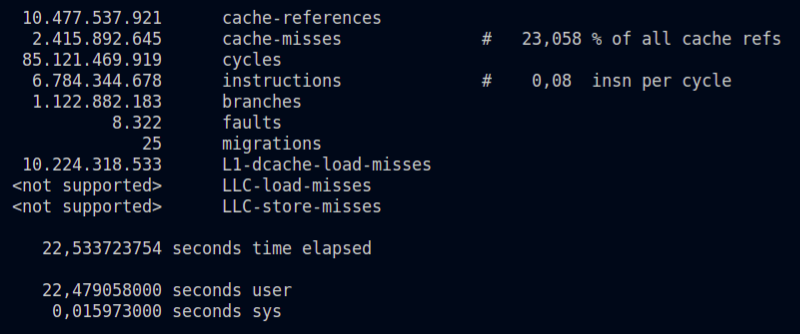
\includegraphics[scale=0.3]{pics/1.png}
  \caption{First performances stats}
  \label{}
\end{figure}


The LLC-load/store-misses stats are not supported in my machine, which is not a big deal in my opinion as what matters to obserrve/inhance our code is the overall number of misses and the the lower cache L1 in particular. They are closer to use and thus provide quicker results when variables are hit (i.e accessed and not missed).

As expected, the given code is not optimized and the access to memory is expensive as shown by the big number of cache misses (i.e 2.5 billions). The whole matrix product calculation is done in about 22 seconds for a total number of cycles of around 79 billions cycles. The machine cycle is a 4 process cycle that includes reading and interpreting the machine language, executing the code and then storing that code.

\begin{figure}[h!]
  \center 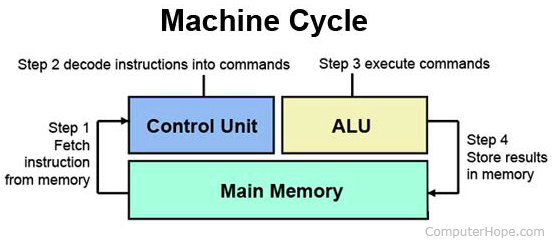
\includegraphics[scale=0.3]{pics/cycle.png}
  \caption{Machine cycle \cite{2}}
  \label{}
\end{figure}

\newpage

\subsection{Detailed records}
In order to avoid any "perf" restrictions one can run as root. Thanks to the "DCMAKE BUILD TYPE=RelWithDebInfo" compiling mode, it is  possible to record the information related to the execution and to generate reports to see the result per function (or even per instruction). By running the command perf record -e cache-misses ./matrix -no-optim followed by perf annotate, we can look at the longuest instructions in the given code.

\begin{figure}[h!]
  \center 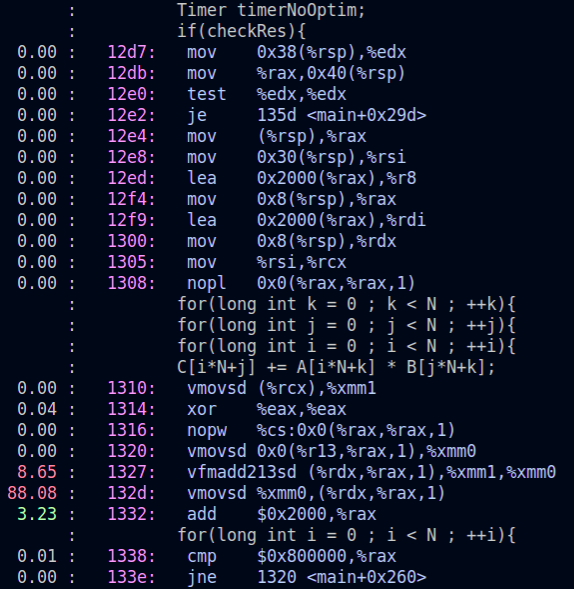
\includegraphics[scale=0.3]{pics/2.png}
  \caption{Performance detailed stats}
  \label{}
\end{figure}


As expected, the nested loop is the cause of such bad performance. For each loop we can see in the right side how many percentage of the cache misses compared to the other loops and the final addition.

%%%%%%%%%%%%%%%%%%%%%%%%%%%%%%%%%%%%%%%%%%%%%%%%%%%%%%%%%%%%%%%%%%%%%%%%%%%%%%%%

\section{Improve the kernel}
\subsection{The memory access}

After reversing the indixes in the nested loop (i.e i and k) we obtain better results, as shown the figure below.

\begin{figure}[h!]
  \center 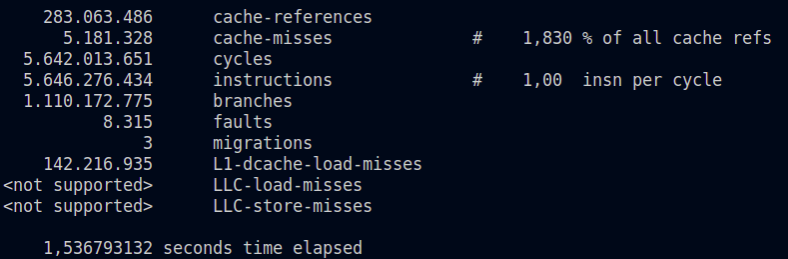
\includegraphics[scale=0.3]{pics/3.png}
  \caption{Performance stats of the first improvement}
  \label{}
\end{figure}

Actually, The arrays can be imagined to be stored in contiguous way in the memory so for better performance the order of loops matters. The execution time fall down to $1.53$ seconds, around $94\%$ improvement. Can we obtain better throughout vectorization and parallelization?

\subsection{Parallelize the code}

A matrix product can be divided in several dot products (i.e line $\times$ column). Thus, we can separate the computation of each dot product between multiple processors working independantly. We use the library OpenMP \cite{3} and its omp pragma instructions. We execute \texttt{OMP\_NUM\_THREADS=i OMP\_PROC\_BIND=TRUE ./matrix -no-check} 8 times, where $i$ will variate between 1 and 8. This is done throughout a script \texttt{par.sh} (see figure below) executed using first chmod +x par.sh then ./par.sh. 

\begin{figure}[h!]
  \center 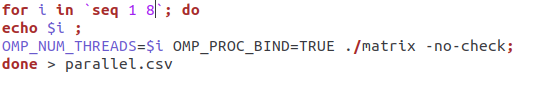
\includegraphics[scale=0.4]{pics/script1.png}
  \caption{Bash script for runnning several commands}
  \label{}
\end{figure}


The results are mainly satisfying but not decreasing at each additional processor parallelization. See figure below.

\begin{figure}[h!]
  \center 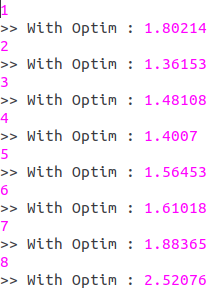
\includegraphics[scale=0.4]{pics/par.png}
  \caption{Parallelization execution time for 1 to 8 processors}
  \label{}
\end{figure}

This unmonotone result might come from the fact that i am using a casual laptop with limited resources.

\subsection{Vectorizing}
For additional enhancement, we use the OpenMP SIMD pragma to vectorize the inner loop. We also do some tests with 1 to 8 processors using the same script (i.e par.sh).

\begin{figure}[h!]
  \center 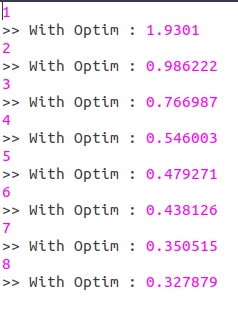
\includegraphics[scale=0.4]{pics/vec.png}
  \caption{vectorization execution time for 1 to 8 processors}
  \label{}
\end{figure}

The results are even better than the previous optimization. A final execution time of 0.32 seconds using 8 processors.
%%%%%%%%%%%%%%%%%%%%%%%%%%%%%%%%%%%%%%%%%%%%%%%%%%%%%%%%%%%%%%%%%%%%%%%%%%%%%%%%


%%%%%%%%%%%%%%%%%%%%%%%%%%%%%%%%%%%%%%%%%%%%%%%%%%%%%%%%%%%%%%%%%%%%%%%%%%%%%%%%

\section{Conclusion}
Using 8 processors, we gained around $99\%$ compared to the badly implemented matrix product version by optimizing the memory access, parallelizing and then vectorizing. My machine is not a good demonstration of such optimization but still one can see the difference for a simple $1024\times1024$ matrix product. Here is a final overview of the perf stats regarding the proposed vectorized solution using only 2 processors.
\newpage
\begin{figure}[]
  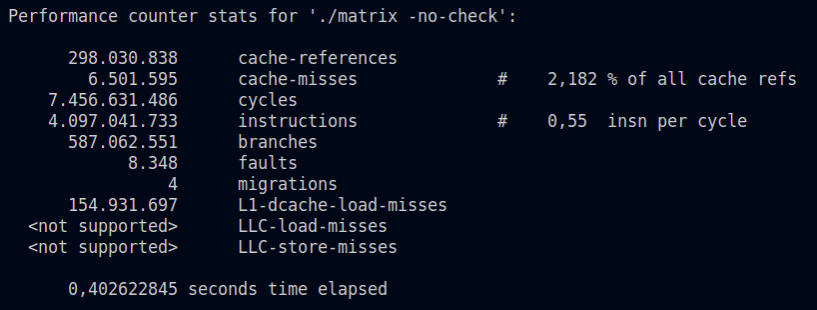
\includegraphics[scale=0.3]{pics/final.png}
  \caption{Final performances}
  \label{}
\end{figure}


It is clear that we have less instructions, less cycles, less migration and most of all less cache misses. Using only 2 processors we reached en execution time of 0.4 seconds instead of 22 seconds for the bad version. Optimizing might take too much time from the developper but it is worth it!
%%%%%%%%%%%%%%%%%%%%%%%%%%%%%%%%%%%%%%%%%%%%%%%%%%%%%%%%%%%%%%%%%%%%%%%%%%%%%%%%

\bibliographystyle{abbrv} % plain
\nocite{*}
\bibliography{report}%


\end{document}
